% The SHA-3 data model [FIPS 202, §3.1, Appendix B.1]: message bytes are read least significant
% bit first, and a 64-bit lane holds eight consecutive bytes in little-endian order.
% Original drawing for the Hash library.
\documentclass[tikz,border=6pt]{standalone}
\usepackage[T1]{fontenc}
\usepackage{lmodern}
% Shared style for the Hash diagrams.
% Palette: Okabe–Ito (colour-blind safe). Every diagram is drawn on an opaque white card so it
% stays legible on dark page themes.
\usetikzlibrary{arrows.meta,positioning,calc,fit,backgrounds}
\definecolor{hsblue}{HTML}{0072B2}
\definecolor{hsorange}{HTML}{E69F00}
\definecolor{hsgreen}{HTML}{009E73}
\definecolor{hsvermilion}{HTML}{D55E00}
\definecolor{hspurple}{HTML}{CC79A7}
\definecolor{hsink}{HTML}{1F2933}
\tikzset{
  >={Stealth[length=2.2mm]},
  every node/.style={font=\sffamily\small, text=hsink},
  wire/.style={draw=hsink, line width=0.6pt, ->},
  reg/.style={draw=hsink, line width=0.6pt, fill=hsblue!12, minimum width=9mm, minimum height=7mm},
  fn/.style={draw=hsink, line width=0.6pt, fill=hsorange!25, rounded corners=2pt, minimum width=10mm, minimum height=6mm},
  input/.style={draw=hsink, line width=0.6pt, fill=hsgreen!20, minimum width=9mm, minimum height=6mm},
  add/.style={circle, draw=hsink, line width=0.6pt, fill=white, inner sep=0pt, minimum size=5mm, font=\sffamily\bfseries},
  card/.style={fill=white, rounded corners=4pt},
}

\begin{document}
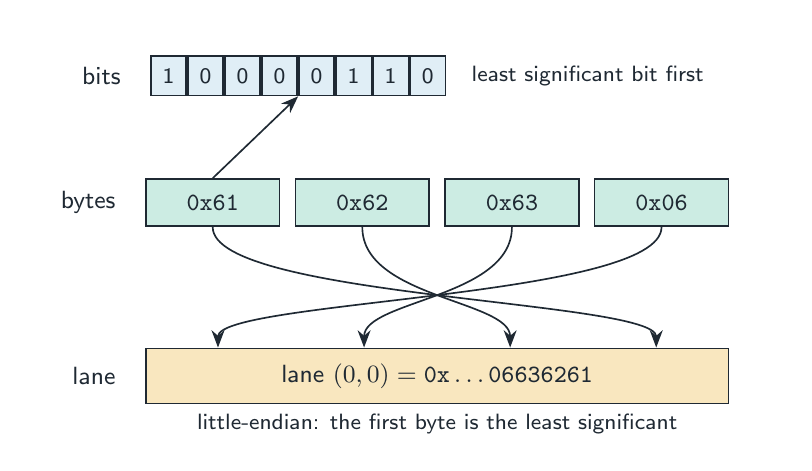
\begin{tikzpicture}
  \def\bw{1.9}
  \foreach \v [count=\i from 0] in {0x61,0x62,0x63,0x06} {
    \node[input, minimum width=17mm] (B\i) at (\i*\bw, 0) {\texttt{\v}};
  }
  \node[anchor=east] at ($(B0.west)+(-0.25,0)$) {bytes};
  % The bits of the first byte, least significant first.
  \foreach \x [count=\j from 0] in {1,0,0,0,0,1,1,0} {
    \node[reg, minimum width=4.5mm, minimum height=5mm, inner sep=0pt] (b\j)
      at ($(B0.north west)+(0.3+\j*0.47,1.3)$) {\footnotesize\x};
  }
  \node[anchor=east] at ($(b0.west)+(-0.25,0)$) {bits};
  \draw[wire] (B0.north) -- ($(b0.south)!0.5!(b7.south)$);
  \node[anchor=west, font=\sffamily\footnotesize] at ($(b7.east)+(0.2,0)$)
    {least significant bit first};
  \node[reg, minimum width=4*\bw cm - 2mm, fill=hsorange!25] (L)
    at ($(B0)!0.5!(B3)+(0,-2.2)$) {lane $(0,0) = \mathtt{0x\ldots06636261}$};
  \node[anchor=east] at ($(L.west)+(-0.25,0)$) {lane};
  \foreach \i in {0,1,2,3} {
    \draw[wire] (B\i.south) .. controls +(0,-0.9) and +(0,0.6) .. ($(L.north east)!{(\i+0.5)/4}!(L.north west)$);
  }
  \node[anchor=north, font=\sffamily\footnotesize] at (L.south)
    {little-endian: the first byte is the least significant};
  \begin{scope}[on background layer]
    \node[card, fit=(B0)(B3)(L)(b0), inner sep=10pt, xshift=-4mm, minimum width=9.6cm] {};
  \end{scope}
\end{tikzpicture}
\end{document}
